%
% erwartung.tex -- Zufallsvariable, Erwartung und Varianz
%
% (c) 2006-2015 Prof. Dr. Andreas Mueller, Hochschule Rapperswil
%
\rhead{Zufallsvariable, Erwartung und Varianz}
\chapter{Zufallsvariable und Erwartungswert} \label{chapter-erwartungswert-und-varianz}

Bis jetzt hat uns nur das Eintreten von Ereignissen interessiert, und
der entwickelte Formalismus war auch nur darauf ausgelegt.
In der Praxis sind aber vor allem auch Experimente wichtig, die
Zahlenwerte als Versuchsausgänge liefern.
Jede Messung kann also ein solches Experiment verstanden werden.

Zahlenwerte entstehen aber auch, wenn man ein Experiment wiederholt
durchführt und als Versuchsausgang die Häufigkeit des Eintretens
eines Ereignisses wählt, also wieder eine Zahl.
In diesem Fall treten natürlich nur ganzzahlige Resultate auf.

Der Ereignis-Formalismus kann uns bestenfalls die Wahrscheinlichkeit
dafür liefern, dass ein Messwert in ein bestimmtes Intervall fällt.
Er kann uns aber nicht helfen die folgenden Fragen zu beantworten:
\begin{enumerate}
\item Mit welchem ungefähren Wert kann man bei der Durchführung der
Messung rechnen?
Wiederholte Messungen werden nicht immer exakt den selben Wert liefern,
sie werden um einen ``Erwartungswert'' streuen.
\item Wie breit ist die Streuung? Gibt es eine Masszahl, mit der man
die Streuung angeben kann, und was bedeutet sie genau?
\end{enumerate}
Um diese Fragen beantworten zu können, müssen wir unserem Modell
der Ereignisse und Wahrscheinlichkeiten zunächst 
ein Modell für den Messprozess anfügen.
Das Konzept der Wahrscheinlichkeit müssen wir sodann feiner ausgestalten,
um einen ``Erwartungswert'' daraus ableiten zu können.
Das gleiche Konzept wird uns auch dazu dienen, eine Masszahl für
die Streuung zu entwickeln, und daraus bereits eine Anzahl interessanter
Anwendungen zu konstruieren.
Es wird aber nicht genügend, die genaue Bedeutung des Streumasses
zu klären, dazu müssen wir mehr über die Verteilung der Wert wissen,
was wir erst im nächsten Kapitel im Detail tun werden.

\section{Zufallsvariable}
In einem Experiment, das mit Hilfe des Ohmschen Gesetzes der Widerstand eines
Bauteils ermitteln soll, wird ein Strom durch das Bauteil geleitet und die
darüber abfallende Spannung gemessen.
Der Versuchsausgang ist also mindestens ein Paar $\omega=(U,I)$ von Spannung und
Strom, möglicherweise aber auch noch mehr, zum Beispiel die Temperatur, die
auch noch gemessen wurde.
Der Versuchsausgang ist also keine Zahl, aber es lassen sich daraus zwei
Zahlen ableiten.
Zu jedem Versuchsausgang $\omega$ gibt es die Zahlen $U(\omega)$
und $I(\omega)$, die in diesem Versuch gemessenen Spannung und der Strom.

Roulette als das Glücksspiel par excellence besteht aus einzelnen
Spielen, in denen jeweils eine Kugel im Roulettekessel in eines von
37 Fächern fällt.
Der Versuchsausgang ist also eine ganze Zahl zwischen $0$ und $36$.
Für den Spieler ist diese Zahl jedoch nur mittelbar von Bedeutung.
Ihn interessiert vor allem, ob die Chips, die er auf dem Roulette-Tisch
gesetzt hat, etwas gewonnen haben, ob als für einen Chip das Ereignis
``Einsatz gewinnt'' eingetreten ist.
Nach den Regeln des Spiels kann man dann aus dem Versuchsausgang den
Gewinn des Spielers ableiten.

Zahlen, die am Ende eines Zufallsprozesses stehen, können also durch
folgendes Modell beschrieben werden.
Zunächst wird ein Experiment durchgeführt, bei welchem wie bisher
ein Versuchsausgang $\omega$ aus den möglichen Versuchsausgängen $\Omega$
ausgewählt wird.
Dann wird aus dem Versuchsausgang über einen deterministischen Prozess
eine Zahl $X(\omega)$ abgeleitet.

\begin{definition}
\index{Zufallsvariable}
\index{Zufallsvariable!stetige}
\index{Zufallsvariable!diskrete}
Eine {\em Zufallsvariable} ist eine Funktion $\Omega\to\mathbb R$.
Eine {\em diskrete} Zufallsvariable nimmt nur diskrete Werte in $\mathbb R$ an.
Bei einer {\em stetigen} Zufallsvariable sind beliebige Werte $X(\omega)\in\mathbb R$
möglich.
\end{definition}

Mit einer Zufallsvariablen $X\colon\Omega\to\mathbb R$ kann man wieder
neue Ereignisse definieren
\begin{align*}
\{X=a\}&=\{\omega\in\Omega\,|\,X(\omega)=a\}
\\
\{a<X\le b\}
&=
\{\omega\in\Omega\,|\, a<X(\omega)\le b\}.
\end{align*}
Bei einer stetigen Zufallsvariable sind die Ereignisse der Form
$\{X=a\}$ nur von beschränktem Nutzen, da nur ganz wenige Versuche
dazu führen werden, dass das Ereignis eintritt.

\subsection{Wurf eines Würfels}
Wirft man einen Würfel, zeigt dieser ein Bild mit einem oder mehreren Punkten, 
dies sind die Elementarereignisse:
\[
\Omega = \{
\epsdice{1},
\epsdice{2},
\epsdice{3},
\epsdice{4},
\epsdice{5},
\epsdice{6}
\}.
\]
Leute, die Zahlen kennen, können diese Bilder auch als Zahlen interpretieren.
Sie verwenden die Abbildung
\[
X\colon \Omega \to \{1,2,3,4,5,6\}
\]
mit den Werten
\begin{align*}
\epsdice{1}&\mapsto 1,\\
\epsdice{2}&\mapsto 2,\\
\epsdice{3}&\mapsto 3,\\
\epsdice{4}&\mapsto 4,\\
\epsdice{5}&\mapsto 5,\\
\epsdice{6}&\mapsto 6.
\end{align*}
Dass diese Zuordnung von Elementarereignissen zu Zahlenwerten tatsächlich
ein zusätzlicher Schritt ist, sieht man zum Beispiel auch daran, dass
in Spielen für Kinder, die die Zahlen noch nicht kennen, Farbwürfel
verwendet werden, und keine Zuordnung von Zahlenwerten vorgenommen wird.

Die Menge $\Omega$ der Elementarereignisse beschreibt alle möglichen Würfe
des Würfels.
Wenn wir uns nur für die gezeigte Augenzahl interessieren,
brauchen wir eine Funktion, welche jedem Elementarereignis diesen speziellen
Ausgang zuordnet:
\[
X: \Omega\to{\mathbb Z}: \omega\mapsto X(\omega).
\]
Eine solche Abbildung heisst eine Zufallsvariable.
Mit Hilfe der Zufallsvariable kann man jetzt das Ereignis, dass eine Sechs
gewürfelt wurde, auch so formulieren:
\[
A_6=\{\omega\in\Omega\;|\;X(\omega) = 6\}.
\]
In $\mathbb{Z}\subset\mathbb{R}$ kann natürlich gerechnet werden, und
auch eine intuitive Vorstellung davon, was ``im Mittel'' etwa heissen
könnte, ist bereits vorhanden.

\subsection{Ein technisches Detail}
Wir hatten früher bemerkt, dass die Menge aller Teilmengen nicht unbedingt
als die Menge der Ereignisse geeignet ist, und dazu die Menge
$\cal A$ der Ereignisse eingeführt.
Wenn aber nicht alle Teilmengen von $\Omega$ Ereignisse sind,
dann ist auch nicht automatisch sichergestellt, dass die
Mengen $\{X < a\}$ für jeden Wert von $a$  Ereignisse sind.
Die technisch korrekte Definition einer Zufallsvariablen ist daher:

\begin{definition}
Eine Zufallsvariable $X$ ist eine Funktion $X\colon \Omega\to \mathbb R$,
die zusätzlich die Eigenschaft hat, dass die Mengen 
$\{\omega | X(\omega) < x\}$ Ereignisse sind.
\end{definition}

Für unsere Zwecke hat dieses Detail keine Konsequenzen, da alle Zufallsvariablen,
die wir betrachten, diese Bedingung automatisch erfüllen.

\subsection{Rechnen mit Zufallsvariablen}
Selbstverständlich können Zufallsvariable auch andere Wertebereiche haben.
Eine Abbildung $X:\Omega\to W$ ist eine $W$-wertige Zufallsvariable.
Alle Operationen im Wertebereich sind auch für Zufallsvariable möglich.
Kann man im Wertebereich $W$ addieren, dann ist auch die Summe zweier
Zufallsvariable $X_1$ und $X_2$ definiert durch
\[
X_1+X_2:\Omega\to W:\omega\mapsto(X_1+X_2)(\omega) := X_1(\omega) + X_2(\omega),
\]
und entsprechend für alle anderen Operationen in $W$.

Bei einer analogen Messung ist zum Beispiel jeder beliebige reelle
Wert möglich, eine reelle Zufallsvariable wäre demnach eine Abbildung
\[
X:\Omega\to\mathbb R:\omega\mapsto X(\omega)\in\mathbb R.
\]
Die Messung von Strom und Spannung an einem Verbraucher definiert zwei
Zufallsvariable $I:\Omega\to\mathbb R$ und $U:\Omega\to \mathbb R$.
Die vom Verbraucher verbrauchte Leistung ist die Zufallsvariable
\[
U\cdot I:\Omega\to\mathbb R: \omega\mapsto (U\cdot I)(\omega) = U(\omega)I(\omega).
\]
Eine komplexe Zufallsvariable wäre die Impedanz
\index{Impedanz}
\[
Z:\Omega\to\mathbb C:\omega\mapsto Z(\omega)\in\mathbb C,
\]
Realteil $\operatorname{Re}Z$ und Imaginärteil $\operatorname{Im}Z$
sind ebenfalls zwei Zufallsvariablen,
für die $Z=\operatorname{Re}Z + i \operatorname{Im}Z$ gilt.

\section{Erwartungswert} \label{section-erwartungswert}
\index{Erwartungswert}
\subsection{Motivation}
\subsubsection{Gewinn beim Münzwurf}
Wir spielen das folgende einfache Wahrscheinlichkeitsexperiment.
In jeder Runde setzen wir einen Einsatz von einem Franken auf den
Ausgang ``Kopf'' oder ``Zahl'' des Wurfes mit einer fairen Münze.
Setzen wir richtig, erhalten wir den Einsatz zurück, zeigt die
Münze das andere Resultat, verlieren wir den Einsatz.
Die Zufallsvariable
$X(\omega)$ soll den Gewinn beim Eintreffen des Ereignisses $\omega$
angeben.

Im
langfristigen Mittel erwarten wir, dass wir in etwa der Hälfte
der Fälle gewinnen, in der anderen Hälfte verlieren.
Im Mittel
müssen wir daher davon ausgehen, dass wir pro Münzwurf einen
halben Franken gewinnen.
Der erwartete Gewinn einem einzelnen
Wurf wäre also $E(X)=0.5$.

Wir versuchen dieses Experiment zu formalisieren.
Die zugehörige
Wahrscheinlichkeitsalgebra kennt nur zwei interessante Ereignisse,
$\{\text{``Kopf''}\}$ oder $\{\text{``Zahl''}\}$.
Die Ereignisse, ihre Wahrscheinlichkeiten und wo sinnnvoll
die zu erwartenden Gewinne sind
in der Tabelle \ref{kopfzahlwahrscheinlichkeit} dargestellt.
\begin{table}
\begin{center}
\begin{tabular}{|c|c|c|}
\hline
Ereignis&Wahrscheinlichkeit&Gewinn\\
\hline
$\{\text{``Kopf''}\}$&0.5&0\\
$\{\text{``Zahl''}\}$&0.5&1\\
$\emptyset$&0&\\
$\Omega$&1&\\
\hline
\end{tabular}
\end{center}
\caption{Wahrscheinlichkeit und Gewinn bei ``Kopf oder Zahl''
\label{kopfzahlwahrscheinlichkeit}}
\end{table}
Die beiden Ereignisse $\{\text{``Kopf''}\}$ und $\{\text{``Zahl''}\}$
decken offenbar alle Möglichkeiten ab, und innerhalb des Ereignisses
ist der Gewinn einheitlich.
Der erwartete Gewinn ist also:
\[
E(\text{``Gewinn''})=\text{``Gewinn bei Kopf''}\cdot P(\text{``Kopf''})
+\text{``Gewinn bei Zahl''}\cdot P(\text{``Zahl''})
\]
Wenn etwas allgemeiner ein Spiel in $n$ verschiedene mögliche
Ausgänge (Ereignisse) $A_i$ unterteilt werden kann, die je den
Gewinn $g_i$ liefern, dann ist der erwartete Gewinn
\[
E=\sum_{i=1}^{n}g_iP(A_i).
\]

\subsubsection{Notenschnitt}
Im Beispiel des Schülers müssten wir also zunächst Ereignisse
identifizieren, und den Gewinn bestimmen, den der Schüler hat, wenn
dieses Ereignis eintritt.
Das Ereignis $A_n=\{\text{``Note $n$''}\}$
beschreibt den Fall, dass der Schüler die Note $n$ erreicht hat.
Aus den experimentellen Daten leiten wir ab, dass die Wahrscheinlichkeiten
für die einzelnen Ereignisse die folgenden sind:
\begin{align*}
P(A_1)&=0\\
P(A_2)&=0\\
P(A_3)&=\frac35\\
P(A_4)&=0\\
P(A_5)&=\frac15\\
P(A_6)&=\frac15\\
\end{align*}
Als
``Gewinn'' beim Eintreten des Ereignisses können wir die Note
ansehen, d.~h.~der Erwartungswert ist 
\[
E=\frac35\cdot 3 + \frac15\cdot 5 + \frac15\cdot 6=\frac{3\cdot 3+ 1\cdot5 + 1\cdot6}{5},
\]
also genau das, was der ``Notendurchschnitt'' auch angibt.

\subsection{Erste Definition und Rechenregeln}
Diese Beispiele führen uns auf folgende abstrakte Definition,
die in den folgenden Abschnitten konkretisiert werden soll.

\begin{definition}
Sei $X$ eine Funktion auf $\Omega$, und lasse sich $\Omega$ in endlich
viele Ereignisse $A_i$ zerlegen, auf denen $X(\omega)$ konstant ist,
dann ist der {\bf Erwartungswert} von $X$
\[
E(X)=\sum_{i=0}^nP(A_i)\cdot X(A_i)
\]
\end{definition}
Aus der Definition lassen sich unmittelbar folgende Rechenregeln ableiten:
\begin{satz}
\label{rechenregeln-erwartungswert}
Sind $X$ und $Y$ Zufallsvariable mit Werten in $\mathbb{R}$ ,
und $\lambda\in\mathbb{R}$, dann gilt
\begin{enumerate}
\item $E(X+Y)=E(X)+E(Y)$
\item $E(\lambda X)=\lambda E(X)$
\item Sei $\chi_A$ die charakteristische Funktion des Ereignisses $A\in{\cal A}$,
welche definiert ist durch
\[
\chi_A\colon\Omega\to\mathbb{R}:\omega\mapsto\begin{cases}
1&\omega\in A\\
0&\omega\not\in A,\\
\end{cases}
\]
dann gilt $E(\chi_A)=P(A)$.
\end{enumerate}
\end{satz}
Während die Definition ziemlich starke Einschränkungen an die Zufallsvariablen
macht, für die der Erwartungswert berechnet werden kann, können
im Satz ausgedrückten Eigenschaften die Basis für eine allgemeinere
Definition sein.
Ob nun der Erwartungswert aus der Vorstellung der Definition
entwickelt wird, oder auf Grund der Eigenschaften des Satzes konstruiert
wird, ist für die Anwendung weiter nicht wesentlich.

\subsection{Erwartungswert bei diskreten Zufallsvariablen}
In einem diskreten Wahrscheinlichkeitsraum ist es möglich, jedem
Elementarereignis eine Wahrscheinlichkeit zuzuschreiben, da die
einelementige Menge $\{\omega\}$ auch ein Ereignis ist.
Wenn man
die Elementarereignisse auch noch aufzählen kann, dann kann man
auch den Erwartungswert einfach berechnen:
\[
E(X)=\sum_{i=0}^\infty X(\omega_i)\cdot P(\{\omega_i\}).
\]
\index{Erwartungswert}
\subsubsection{Erwartete Augenzahl beim Würfeln mit einem Würfel}
Wir beschreiben des Würfeln mit einem Würfel mit Hilfe der
Elementarereignisse $\Omega=\{1,2,3,4,5,6\}$.
Offenbar handelt es sich
hier um einen diskreten Wahrscheinlichkeitsraum, in dem jedes
Elementarereignis die Wahrscheinlichkeit $\frac16$ hat.
Die Funktion
$X$ liefert die Augenzahl, also $X(i)=i$.
Die erwartete Augenzahl
ist also
\begin{align*}
E(X)&=
1\cdot\frac16+
2\cdot\frac16+
3\cdot\frac16+
4\cdot\frac16+
5\cdot\frac16+
6\cdot\frac16\\
&=\frac{1+2+3+4+5+6}6\\
&=\frac{21}{6}=3.5.
\end{align*}
\subsubsection{Erwartete Augenzahl beim Würfeln mit zwei Würfel}
Auch hier liegt ein diskreter Wahrscheinlichkeitsraum vor, dessen
Elementarereignisse die Paare $(i,j)$ sind, mit $1\le i,j\le 6$.
Die Wahrscheinlichkeit jedes einzelnen Paares ist $\frac1{36}$.
Die Funktion $X$ ist jetzt $X(i,j)=i+j$.
Der Erwartungswert ist
also
\begin{align*}
E(X)&=\sum_{i=1}^6\sum_{j=1}^6\frac{i+j}{36}
=\frac1{36}\sum_{i=1}^6\sum_{j=1}^6(i+j)
=\frac1{36}\sum_{i=1}^6\bigl(6i + \sum_{j=1}^6j\bigr)\\
&=\frac1{36}\sum_{i=1}^6(6i + 21)
%=\frac1{36}\bigl(6\sum_{i=1}^6i + 21 \bigr)
=\frac1{36}\bigl(6\sum_{i=1}^6i + 6\cdot21 \bigr)\\
&=\frac1{36}(6\cdot 21 + 6\cdot21 )
=\frac1{36}(2\cdot 6\cdot 21)
=\frac1{6}(2\cdot 21)
=7.
\end{align*}
Man kann als im Mittel mit einer Augensumme von 7 rechnen.
Dies ist
gleichzeitig auch der häufigste Wert, dies trifft aber im allgemeinen
nicht zu.

\subsubsection{Erwarteter Gewinn beim Roulette}
\index{Roulette!Gewinnerwartung}
Beim Roulette setzt man seinen Einsatz auf eine Zahl zwischen $0$
und $36$.
Gewinnt die Zahl, bekommt man das 36-fache des Einsatzes,
andernfalls erhält man nichts.
Die Wahrscheinlichkeit jeder einzelnen
Zahl ist gleich gross, nämlich $\frac1{37}$.
Der erwartete Gewinn pro
Franken Einsatz auf die Zahl $x$ ist also
\[
E(G)= \frac1{37}\cdot 36=\frac{36}{37}<1,
\]
man verliert also auf jeden Fall etwas.

Im Roulette gibt es aber weitere Spielmöglichkeiten.
Man kann zum Beispiel
auf rot setzen.
Wie gross ist der erwartete Gewinn in diesem Fall?
Im Falle einer roten Zahl gewinnt man den doppelten Einsatz,
im Falle einer schwarzen Zahl oder der Null verliert man den Einsatz.
Da eine rote Zahl mit Wahrscheinlichkeit $\frac{18}{37}$ kommt, ist
die Gewinnerwartung 
\[
E(G)=\frac{18}{37}\cdot 2=\frac{36}{37}<1.
\]
"Ahnliches geschieht, wenn man vier Zahlen setzt.
Kommt eine der Zahlen,
gewinnt man das neunfache des Einsatzes, sonst ist der Einsatz 
verloren.
Die Gewinnerwartung ist wieder
\[
E(G)=\frac{4}{37}\cdot 9=\frac{36}{37}<1.
\]
Wie auch immer man es anstellt, man erhält im Mittel in jedem Spiel
weniger zurück als man eingesetzt hat.

\subsubsection{Erwarteter Gewinn beim Lotto}
\index{Lotto!Gewinnerwartung}
Beim Lotto werden $k$ Zahlen aus $N$ möglichen Zahlen gezogen.
Wenn dabei die Zahlenkombination gezogen wird, auf die man getippt
hat, gewinnt man den Hauptgewinn und den Jackpot, diesen Betrag bezeichnen
wir mit $G$.
Da die Fälle mit
weniger als sechs Richtigen nicht so viel hergeben, berechnen wir
nur den erwarteten Gewinn für sechs Richtige.

Die Ereignisalgebra für dieses Problem besteht also aus 
6-Tupeln von Zahlen, die die Lottomaschine am Wochenende ermittelt:
\[
\Omega=\{(a_1, a_2, a_3, a_4, a_5, a_6)\;|\;1\le a_i\le 45, a_i\ne a_j\}.
\]
Dabei kann natürlich niemals eine Zahl doppelt auftreten.
Das Ereignis $A$, welches den Hauptgewinn bringt, enthält alle
Elementarereignisse, die genau die Zahlen auf dem Lottozettel des
Gewinners enthalten.
Da die Lottomaschine die Zahlen in irgend einer
Reihenfolge produziert, enthält dieses Ereignis $6!$ Elementarereignisse.
Insgesamt hat $\Omega$ $N(N-1)(N-2)(N-3)(N-4)(N-5)$ Elemente, somit ist
die Wahrscheinlichkeit, dass man gewinnt:
\[
P(A)=\frac{6!}{N(N-1)(N-2)(N-3)(N-4)(N-5)}.
\]
Damit
kann man den erwarteten Gewinn ausrechnen:
\[
E(X) = P(A)\cdot G.
\]
Erst wenn dieser Betrag den Einsatz für ein einzelnes Spiel übersteigt,
ist Lottospielen rational begründbar.
Da $P(A)$ unverändert ist,
ist dazu notwendig, dass $G$ gross wird.
Da nur die Hälfte der
Einzahlungen überhaupt wieder zur Auszahlung gelangt, ist dies nur
möglich, wenn der Jackpot gross ist.
Ein grosser Jackpot zieht natürlich
auch mehr Gelegenheitsspieler an, was $G$ ebenfalls vergrössert.
\subsubsection{Niedrigere Gewinnklassen}
Natürlich
haben wir hier die niedrigeren Gewinnklassen (5 Richtige, 4 Richtige
etc.~vernachlässigt).
Um diese zu berechnen betrachten wir die folgende
Ereignisalgebra.
Elementarereignisse sind $n$-elementige Teilmengen von
$\{1,\dots,N\}$, davon gibt es $\binom{N}{n}$.
Uns interessiert das Ereignis
\[
A_k=\{\omega\;|\;|\omega\cap A|=k\},
\]
also diejenigen Elementarereignisse, die genau $k$ Elemente aus der
$M$-elementigen Teilmenge
$A\subset\Omega$ haben.
Im Beispiel des Lottos sind $A$ die Zahlen, die
auf dem Lottozettel angekreuzt sind.
Dazu müssen offenbar zunächst $k$ Zahlen aus $A$ ausgewählt werden,
und dann noch $n-k$ Zahlen aus $\Omega\setminus A$.
Ersteres ist
auf $\binom{|A|}{k}$ Arten möglich, letzteres auf $\binom{N-|A|}{n-k}$
Arten.
Insgesamt gibt es also 
\[
\binom{M}{k}\binom{N-M}{n-k}
\]
Elementarereignisse, die genau $k$ Elemnte in $A$ haben.
Insgesammt gibt es $\binom{N}{n}$.
Die Wahrscheinlichkeit,
in einem Lotto $k$ richtige
zu treffen, bei dem man auf dem Lottozettel $M$ zahlen ankreuzen kann,
und bei dem aus $N$ Zahlen $n$ gezogen werden, ist somit
\begin{equation}
h(k|N;M;n)=\frac{\binom{M}{k}\binom{N-M}{n-k}}{\binom{N}{n}}.
\label{hypergeometrische-verteilung}
\end{equation}
Dies ist die hypergeometrische Verteilung.
Mit ihr lässt sich jetzt der erwartete
Gewinn berechnen, man muss nur noch den Gewinn in jeder Klasse kennen.
Ist $G_k$ der Gewinn in der Klasse ``$k$ richtige'', dann ist der
erwartete Gewinn:
\[
E(G)=\sum_{k=0}^{6}h(k|N;M;n)G_k.
\]

\subsection{Erwartungswert und Messungen} \label{erwartungswertvonmesswerten}
\index{Erwartungswert!von Messungen}
In der Tabelle \ref{widerstandswerte} sind die Resultate der Messung des
Widerstandes zufällig eingekaufter 1k$\Omega$-Widerstände aufgeführt.
Im Kapitel 1 wurde gezeigt, dass die Mess\-werte nicht den exakten Wert
des Widerstands wiedergeben, sondern nur ein Intervall.
Eine Messung ist
also eigentlich eine Zufallsvariable, welche dem zufällig ausgewählten
Widerstand $\omega$ seinen Wert $R(\omega)$ zuordnet.
Das Messgerät zeigt
dann an, welches der Ereignisse $R^{-1}(I)$ realisiert worden ist.
Bei der Widerstandsmessung geschah dies mit folgenden Häufigkeiten:
\begin{center}
\begin{tabular}{|c|c|c|}
\hline
Ereignis&Häufigkeit&Wahrscheinlichkeit\\
\hline
$[0.989,0.990)$&6&0.30\\
$[0.990,0.991)$&7&0.35\\
$[0.991,0.992)$&5&0.25\\
$[0.982,0.993)$&2&0.10\\
\hline
\end{tabular}
\end{center}
Die Zufallsvariable $R$ hat damit folgenden Mittelwert:
\begin{align*}
E(R)&=p([0.989,0.990))\cdot 0.989+
p([0.990,0.991))\cdot 0.990\\
&\qquad  +
p([0.991,0.992))\cdot 0.991+
p([0.982,0.993))\cdot 0.992\\
&=
0.3\cdot 0.989+
0.35\cdot 0.990+
0.25\cdot 0.991+
0.1\cdot 0.992\\
&=0.99015.
\end{align*}

\subsection{Unabhängigkeit und Produktregel}
\index{Erwartungswert!Unabh\ängigkeit}
Für die Wahrscheinlichkeit eines Schnittereignisses $P(A\cap B)$ galt die
Produktformel
\[
P(A\cap B)=P(A)\cdot P(B)
\]
nur unter der zusätzlichen Bedingung, dass die Ereignisse $A$ und $B$
unabhängig sind.
Demzufolge ist auch für den Erwartungswert eines
Produktes $E(XY)$ zweier Zufallsvariablen zu erwarten, dass zusätzliche
Voraussetzungen gemacht werden müssen, um $E(XY)$ berechnen zu können.

\begin{figure}
\begin{center}
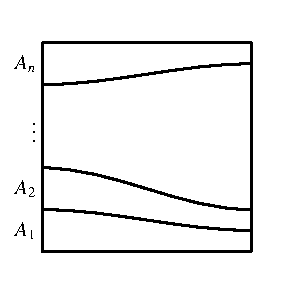
\includegraphics[width=0.3\hsize]{images/erwartung-4}
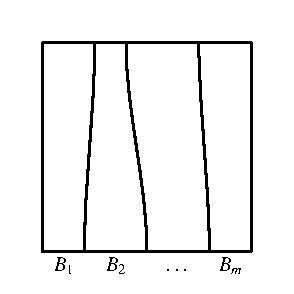
\includegraphics[width=0.3\hsize]{images/erwartung-3}
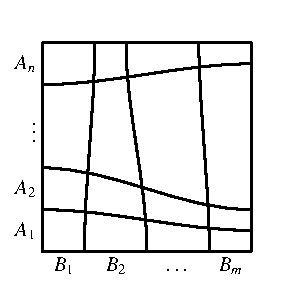
\includegraphics[width=0.3\hsize]{images/erwartung-2}
\end{center}
\caption{Ereignisse $A_i$ zur Berechnung von $E(X)$, $B_j$ zur Berechnung
von $E(Y)$ und $A_i\cap B_j$ zur Berechnung von $E(XY)$.
\label{productexpectation}}
\end{figure}
Seien $A_i$ und $B_j$ Ereignisse so, dass $X$ auf den $A_i$ und $Y$ auf
den $B_j$ konstant ist.
Dann kann man die Ereignisse $A_i\cap B_j$
zur Berechnung des Erwartungswertes heranziehen, wie in
Abbildung~\ref{productexpectation}, denn auf ihnen ist sowohl $X$ wie
auch $Y$ konstant.
Die Wahrscheinlichkeit von $A_i\cap B_j$ kann aber nur dann
durch die Wahrscheinlichkeiten von $A_i$ und $B_j$ ausgedrückt werden,
wenn die Ereignisse $A_i$ und $B_j$ paarweise
unabhängig sind.
Dann berechnet man:
\begin{align*}
E(XY)&=\sum_{i=1}^n\sum_{j=1}^m X(A_i\cap B_j)Y(A_i\cap B_j)P(A_i\cap B_j)\\
&=\sum_{i=1}^n\sum_{j=1}^m X(A_i)Y(B_j)P(A_i)P(B_j)\\
&=\sum_{i=1}^n X(A_i)P(A_i)\sum_{j=1}^mY(B_j)P(B_j)\\
&=E(X)\cdot E(Y).
\end{align*}
Die oben verwendete Unabhängigkeitsbedingung kann man mit folgender
Definition erzwingen:
\begin{definition}Zwei Zufallsvariable $X$ und $Y$ heissen
unabhängig, wenn die Ereignisse $\{\omega|X(\omega)\le x\}$
und $\{\omega|Y(\omega)\le y\}$ für alle $x,y\in\mathbb R$
unabhängig sind, also
\[
P((X\le x)\wedge(Y\le y))=P(X\le x)\,P(Y\le y)\quad\forall x,y\in\mathbb{R}.
\]
\end{definition}
\index{Produktregel!f\ür den Erwartungswert}
Damit haben wir auch für Zufallsvariable eine Produktregel:
\begin{satz}
\label{produktregel-erwartungswert}
Sind $X$ und $Y$ unabhängige Zufallsvariablen, dann gilt
\[
E(XY)=E(X)\cdot E(Y).
\]
Für zwei beliebige Funktionen $f$ und $g$ von $\mathbb{R}$ nach $\mathbb{R}$,
so dass $f(X)$ und $g(Y)$ immer noch Zufallsvariable sind, gilt
\[
E(f(X)g(Y))=E(f(X))E(g(Y)).
\]
\end{satz}
Seien $X$ und $Y$ die Augenzahlen beim Würfeln mit zwei Würfeln.
Die Ereignisse $X\le x$ und $Y\le y$ sind offensichtlich unabhängig
(``horizontale und vertikale Streifen''), daher gilt
\[
E(XY)=E(X)E(Y)=3.5^2=12.25.
\]

\subsection{Erwartungswert und Integration}
\index{Erwartungswert!und Integration}
Die Berechnung des Erwartungswertes war im vorangegangene Abschnitt
einfach möglich, weil wir annehmen konnten, dass es Ereignisse $A$
gibt, auf denen die Zufallsvariable $X$ konstant ist.
Wenn diese
Bedingung nicht mehr gilt, könnte man versuchen, den Erwartungswert
durch die Summe der kleinsten und grössten möglichen Werte auf jedem
Ereignis $A_i$ einzuschachteln:
\[
\sum_{i=0}^nP(A_i)\min_{\omega\in A_i}X(\omega)
\le E(X)\le
\sum_{i=0}^nP(A_i)\max_{\omega\in A_i}X(\omega).
\]
Wir betrachten als Spezialfall die Ereignisalgebra für eine
Messung, hier ist $\Omega=\mathbb{R}$.
Die Wahrscheinlichkeitsfunktion $P$
liefert zu jedem Teilintervall $I\subset \mathbb{R}$ eine Wahrscheinlichkeit.
Wir betrachten eine Zerlegung der reellen Achse in Teilintervalle $I_i$.
Zu einer Funktion $X\colon \mathbb{R}\to\mathbb{R}$ kann man jetzt den
Erwartungswert wie folgt berechnen:
\[
\sum_{i=0}^nP(I_i)\min_{x\in I_i}X(x)
\le E(X)\le
\sum_{i=0}^nP(I_i)\max_{x\in I_i}X(x).
\]
Diese Konstruktion ist aber aus der Analysis vertraut, auf diese
Art wurde das Integral konstruiert.
Die Summenausdrücke sind sogenannte
Riemannsche Summen, der einzige Unterschied ist, dass nicht die Länge des
Intervalls, sondern die Wahrscheinlichkeit $P(I_i)$ des Intervalls gemessen
wird.
Der Erwartungswert ist also eine Art verallgemeinertes Integral,
wofür der Mathematiker auch 
\[
E(X)=\int_{\Omega}X(\omega)dP(\omega)
\]
schreibt.
Da uns diese Betrachtungsweise keine wirklich praktikablen
Möglichkeiten zur Berechnung von $E(X)$ bietet, verfolgen wir sie
hier nicht weiter, werden aber im nächsten Kapitel eine verwandte
Technik kennen lernen, welche nur gewöhnliche Integrale verwendet.

\section{Varianz}\label{section-varianz}
\index{Varianz}
Die Qualitätskontrolle bei der Herstellung von Widerständen versucht
ein Mass dafür zu entwickeln, wie genau die produzierten Widerstände
den beabsichtigen Widerstandswert einhalten. 
Dazu werden der Produktion einige Widerstände entnommen und ihr Wert
nachgemessen.
Den Erwartungswert des Widerstandswertes kann man mit
Hilfe des Mittelwertes abschätzen, er sollte ungefähr mit dem Sollwert
übereinstimmen.
Wie aber kann man die ``Streuung'' der Widerstandswerte
bewerten?

Als weiteres Beispiel betrachten wir die Zufallsvariable $X$
``Messung einer Spannung''.
Nicht jede Messung ergibt den gleichen Wert,
das Signal ist von einem Rauschen überlagert.
Der Mittelwert der
Messwert entspricht gemäss dem vorangegangenen Abschnitt dem Erwartungswert
$E(X)$.
Wie aber soll das Ausmass des Rauschens gemessen werden?
Ein praktischer Ansatz besteht darin, nach der Energie zu fragen, die
in dem Rauschsignal steckt.
Die Leistung einer Wechselspannung $U(t)$
an einem Widerstand $R$ ist ja
$\frac{U(t)^2}R$, d.~h.~die mittlere Leistung während des Intervalls $[t_0,t_1]$ 
ist
\[
\frac1{t_1-t_0}\int_{t_0}^{t_1}\frac{U(t)^2}R\,dt.
\]
Stellen wir uns vor, dass die Spannungsmessung $X$ in regelmässigen, kurzen
Zeitintervallen wiederholt wird, dann ist die mittlere Leistung
des Differenzsignal $X-E(X)$ also proportional Summe der Quadrate
der Werte $(X-E(X))^2$, oder
\[
E((X-E(X))^2).
\]

\subsection{Definition}
\index{Varianz!Definition}
Die Einführungsbespiele motivieren folgende Definition:
\begin{definition}
Sei $X\colon\Omega\to\mathbb{R}$ eine Zufallsvariable, dann
heisst die durch $\operatorname{var}(X)^2=E((X-E(X))^2)$ definierte Grösse $\operatorname{var}(X)$ die
{\bf Varianz} von $X$.
Es ist insbesondere
\[
\operatorname{var}(X)=E((X-E(X))^2)=E(X^2)-E(X)^2
\]
\end{definition}
Die letzte Gleichung kann man leicht nachrechnen:
\begin{align*}
\operatorname{var}(X)&=E((X-E(X))^2)\\
&=E(X^2-2XE(X)+E(X)^2)\\
&=E(X^2)-2E(X)E(X)+E(X)^2\\
&=E(X^2)-E(X)^2.
\end{align*}
%%
\begin{figure}
\begin{center}
%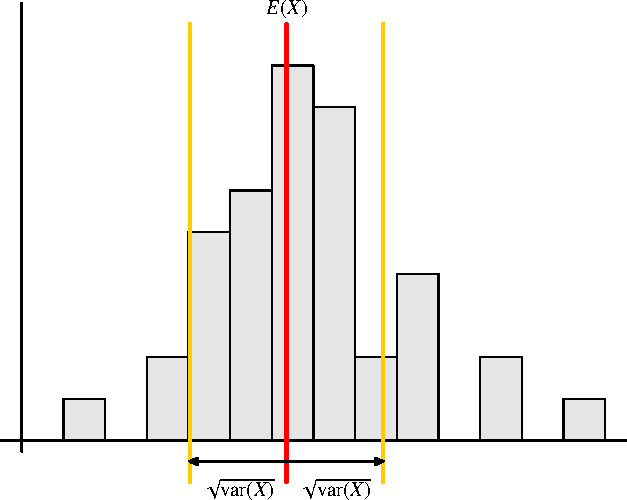
\includegraphics[width=\hsize]{images/erwartung-1}
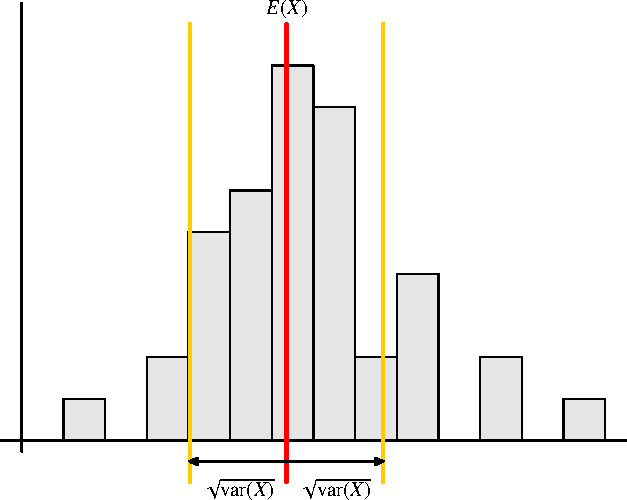
\includegraphics{images/erwartung-1}
\end{center}
\caption{Visualisierung von Erwartungswert und Varianz in einem Histogramm
\label{histogram}}
\end{figure}%

Man beachte, dass $\operatorname{var}(X)$ die Masseinheit des Quadrates
von $X$ hat.
Wenn also $X$ als Masseinheit eine Länge hat,
dann hat $\operatorname{var}(X)$ die Masseinheit einer Fläche.
Insbesondere kann man $\operatorname{var}(X)$ nicht in der gleichen
Zeichnung visualisieren wie $E(X)$.
Aber die Grösse $\sqrt{\operatorname{var}(X)}$ hat die gleiche Masseinheit, sie
drückt die ``Streubreite'' der Werte von $X$ aus,
wie in Abbildung~\ref{histogram} veranschaulicht.

Die Definition der Varianz ``passt'' in natürlicher Weise zum Erwartungswert,
wie der folgende Satz zeigt:
\begin{satz}\label{erwartungswert-charakterisierung}
Der Erwartungswert $E(X)$ einer reellen Zufallsvariable $X$ ist diejenige
reelle Zahl $\mu$, für die $E((X-\mu)^2)$ minimal wird.
\end{satz}
\begin{proof}[Beweis]
Aus den Rechenregeln finden wir
\begin{align*}
E((X-\mu)^2)
&=
E(X^2-2\mu X+\mu^2)
\\
&=
E(X^2)-2\mu E(X) +\mu^2E(1)
\\
&=
E(X^2)-2\mu E(X) +\mu^2
\end{align*}
Dies ist eine quadratische Funktion, die ihren Scheitelpunkt bei $\mu$ hat.
Man kann dies auch durch Nullsetzen der Ableitung nach $\mu$ finden:
\[
\frac{d}{d\mu}\left(E(X^2)-2\mu E(X) +\mu^2\right)=-2 E(X)+2\mu=0,
\]
Auflösen nach $\mu$ ergibt $\mu=E(X)$.
\end{proof}
Wir wenden die Definition der Varianz auf das Beispiel der Widerstandsmessung
an,
Wir haben bereits im Abschnitt \ref{erwartungswertvonmesswerten}
den Erwartungswert $E(R)=0.99015$ der Widerstandsmesswerte ermittelt, darauf aufbauend
können wir jetzt auch die Varianz berechnen.
Man findet zum Beispiel die Widerstandswerte gemäss
Tabelle~\ref{varianzberechnung}.
\begin{table}
\begin{center}
\begin{tabular}{|c|r|r|r|}
\hline
Nummer&Messwert&Abweichung&$\text{Abweichung}^2$\\
\hline
1&0.990&-0.00015&0.0000000225\\
2&0.989&-0.00115&0.0000013225\\
3&0.991&0.00085&0.0000007225\\
4&0.991&0.00085&0.0000007225\\
5&0.991&0.00085&0.0000007225\\
6&0.989&-0.00115&0.0000013225\\
7&0.990&0.00015&0.0000000225\\
8&0.989&-0.00115&0.0000013225\\
9&0.992&0.00185&0.0000034225\\
10&0.992&0.00185&0.0000034225\\
11&0.990&-0.00015&0.0000000225\\
12&0.989&-0.00115&0.0000013225\\
13&0.990&-0.00015&0.0000000225\\
14&0.991&0.00085&0.0000007225\\
15&0.989&-0.00115&0.0000013225\\
16&0.990&-0.00015&0.0000000225\\
17&0.989&-0.00115&0.0000013225\\
18&0.990&-0.00015&0.0000000225\\
19&0.990&-0.00015&0.0000000225\\
20&0.991&0.00085&0.0000007225\\
\hline
&$\mu=1.000$&$\sigma=0.000963$&
$\sigma^2=0.0000009275$\\
\hline
\end{tabular}
\end{center}
\caption{Einzelmessungen an Widerständen und Berechnung der Varianz
\label{varianzberechnung}}
\end{table}

\subsubsection{Beispiel: Wurf einer fairen Münze}
Beim Wurf einer fairen Münze werde der Gewinn $1$ ausbezahlt bei
``Kopf'', bei ``Zahl'' wird hingegen $0$ ausbezahlt.
Es ist klar, dass die erwartete Auszahlung $E(X)=\frac12$ ist.
Daraus lässt sich jetzt auch die Varianz berechnen:
\begin{align*}
\operatorname{var}(X)
&=
E((X-E(X))^2)=E\biggl(\biggl(X-\frac12\biggr)^2\biggr)
=\frac12\cdot \biggl(1-\frac12\biggr)^2+\frac12\biggl(0-\frac12\biggr)^2\\
&=\frac12\cdot\frac14+\frac12\cdot\frac14=\frac14.
\end{align*}

\subsection{Empirische Berechnung}
\index{Varianz!angen\äherte Berechnung}
Wir betrachten das praktische Beispiel der Bestimmung der Varianz
einer Messreihe.
Gegeben sind also die Messwerte $(x_i)_{1\le i\le n}$
Auf den ersten Blick sieht es so aus, als wäre für die Berechnung der Varianz
sehr viel Speicherplatz erforderlich.
Zwar ist für die Berechnung des
Erwartungswertes von $\mu=E(X)=\frac1n\sum_{i=1}^n x_i$ kein besonderer Aufwand
notwendig, da die Summe laufend gebildet werden kann.
Zur Berechnung der
Varianz muss aber erst $\mu$ bestimmt werden, bevor man die Differenzen $(x_i-\mu)$
bilden kann.
Trotzdem lässt sich die Berechnung vereinfachen:
\begin{align*}
E((X-\mu)^2)&=\frac1n\sum_{i=1}^n(x_i-\mu)^2\\
&=\frac1n\sum_{i=1}^n(x_i^2-2\mu x_i+\mu^2)\\
&=\frac1n\sum_{i=1}^nx_i^2-2\mu\frac1n\sum_{i=1}^n x_i+\mu^2\\
&=\frac1n\sum_{i=1}^nx_i^2-\biggl(\frac1n\sum_{i=1}^nx_i\biggr)^2.
\end{align*}
\subsubsection{Beobachtungen}
\begin{enumerate}
\item
Es genügt also, $x_i$ und $x_i^2$ zu summieren, wozu nur zwei Speicherplätze
benötigt werden.
Aus den beiden Summen kann die Varianz bereits berechnet werden.
Es ist nicht nötig, die einzelnen Messwerte $x_i$ zu speichern.
\item
Die Berechnung der Varianz kann also ganz einfach mit einer Tabelle
erfolgen:
\begin{center}
%\begin{tabular}{|>{$}c<{$}|>{$}c<{$}|}
\begin{tabular}{|c|c|c|}
\hline
$i$&$x_i$&$x_i^2$\\
\hline
$1$&$x_1$&$x_1^2$\\
$2$&$x_2$&$x_2^2$\\
$\vdots$&$\vdots$&$\vdots$\\
$n$&$x_n$&$x_n^2$\\
\hline
&$\sum_{i=0}^n x_i$&$\sum_{i=0}^n x_i^2$\\
\hline
\end{tabular}
\end{center}
\item
Grosse Abweichungen können vorkommen, und bekommen wegen des
Quadrates in der Varianz auch grosses Gewicht.
Hat man aber nur
wenige Messwerte, ist es unwahrscheinlich, eine solche grosse
Abweichung, einen ``Ausreisser'', zu sehen.
Daher unterschätzt
diese empirische Formel den tatsächlichen Wert der Varianz immer
dann, wenn $n$ klein ist.
Wir werden später sehen, dass eine
besser Schätzung zu bekommen ist, wenn man noch einen Korrekturfaktor
$\frac{n}{n-1}$ hinzufügt.
\end{enumerate}

\subsection{Weitere Rechenregeln}
\begin{satz}
\label{rechenregeln-varianz}
Seien $X$ und $Y$ unabhängige Zufallsvariable, dann haben
Summe und Produkt folgende Varianz:
\begin{align*}
\operatorname{var}(\lambda X)&=\lambda^2\operatorname{var}(X)\\
\operatorname{var}(X+Y)&=\operatorname{var}(X)+\operatorname{var}(Y)\\
\operatorname{var}(XY)&=\operatorname{var}(X)\operatorname{var}(Y)
+
\operatorname{var}(Y)E(X)^2+\operatorname{var}(X)E(Y)^2.
\end{align*}
\end{satz}
\begin{proof}[Beweis]Durch einfaches Nachrechnen unter Ausnützen der
Rechenregeln für den Erwartungswert und der
Unabhängigkeit von $X$ und $Y$, d.~h.~$E(XY)=E(X)E(Y)$:
\begin{align*}
\operatorname{var}(X+Y)
&=E((X+Y)^2)-E(X+Y)^2\\
&=E(X^2+2XY+Y^2)-(E(X)+E(Y))^2\\
&=E(X^2)+2E(XY)+E(Y^2)-E(X)^2-2E(X)E(Y)-E(Y)^2\\
&=E(X^2)-E(X)^2+E(Y^2)-E(Y)^2\\
&=\operatorname{var}(X)+\operatorname{var}(Y).
\end{align*}
Durch Ziehen der Wurzel folgt die Behauptung aus der letzten Gleichung.
Für das Produkt gilt
\begin{align*}
\operatorname{var}(XY)
&=E(X^2Y^2)-E(XY)^2\\
&=E(X^2)E(Y^2)-E(X)^2E(Y)^2\\
&=(\operatorname{var}(X)+E(X)^2)(\operatorname{var}(Y)+E(Y)^2)
-E(X)^2E(Y)^2\\
&=\operatorname{var}(X)\operatorname{var}(Y)+E(X)^2\operatorname{var}(Y)
+\operatorname{var}(X)E(Y)^2
\end{align*}
und daraus die Behauptung.
\end{proof}

\subsubsection{Beobachtungen}

\begin{enumerate}
\item
Die Varianz funktioniert ähnlich wie das Quadrieren für gewöhnliche Zahlen.
Schreibt man $E(XY)-E(X)E(Y)=\operatorname{cov}(X,Y)$, lautete die
binomische Formel wird für die Varianz:
\begin{equation}
\operatorname{var}(X+Y)=\operatorname{var}(X)
+2\operatorname{cov}(X,Y)
+\operatorname{var}(Y).
\label{var-summe-abhaengig}
\end{equation}
Die Kovarianz $\operatorname{cov}(X,Y)$ spielt also die Rolle des gemischten
Terms in der ``gewöhnliche'' binomischen Formel.
\item
Sind $X$ und $Y$ unabhängig, gilt daher die Formel
\begin{align*}
\operatorname{var}(X+Y)
&=
\operatorname{var}(X)
+
\operatorname{var}(Y),
\\
\sqrt{\operatorname{var}(X+Y)}
&=
\sqrt{
\sqrt{\operatorname{var}(X)}^2
+
\sqrt{\operatorname{var}(Y)}^2
}.
\end{align*}
Die Grössen $\sqrt{\operatorname{var}(X)}$ und $\sqrt{\operatorname{var}(Y)}$
werden daher wie die Katheten eines rechtwinkligen Dreiecks addiert,
man spricht von {\it pythagoräischer} Addition.
\end{enumerate}

\subsubsection{Anwendung: Wurf von \texorpdfstring{$n$}{n} Münzen}
Sei $X$ die Anzahl ``Kopf'' beim Wurf von $n$ Münzen.
Natürlich wird
$X$ nur Werte zwischen $0$ und $n$ annehmen.
Zur Berechnung von $E(X)$ und $\operatorname{var}(X)$ wollen wir
die Rechenregeln verwenden.
Dabei verwenden wir neue Zufallsvariablen
$X_i$ wie folgt:
\begin{center}
\begin{tabular}{clcc}
$X_1$&Anzahl Kopf im ersten Wurf&$E(X_1)=\frac12$&$\operatorname{var}(X_1)=\frac14$\\
$X_2$&Anzahl Kopf im zweiten Wurf&$E(X_2)=\frac12$&$\operatorname{var}(X_2)=\frac14$\\
&$\dots$&&\\
$X_n$&Anzahl Kopf im $n$-ten Wurf&$E(X_n)=\frac12$&$\operatorname{var}(X_n)=\frac14$.
\end{tabular}
\end{center}
Damit kann man Erwartungswert und Varianz von $X=X_1+X_2+\dots+X_n$ berechnen:
\begin{align*}
E(X)&=
E(X_1)+
E(X_2)+\dots+
E(X_n)
=
\frac{1}2+
\frac{1}2+\dots+
\frac{1}2=\frac{n}2,
\\
\operatorname{var}(X)
&=
\operatorname{var}(X_1)
+
\operatorname{var}(X_2)
+\dots+
\operatorname{var}(X_n)
=\frac14+\frac14+\dots+\frac14=\frac{n}4.
\end{align*}

\section{Wie genau ist der Mittelwert?}
Der Erwartungswert drückt aus, wie gross eine Zufallvariable ``im Mittel''
sein wird.
Je grösser aber die Varianz ist, desto grösser wird die Abweichung
der Zufallsvariable vom ``mittleren Wert'' sein.
Wie misst man diese Abweichung? Mit der Varianz haben wir bereits
ein Mass für die mittlere Abweichung, aber noch keinen Hinweis
darauf, wie häufig grosse Abweichungen vorkommen werden.

Sei $\mu=E(X)$ der Erwartungswert der Zufallsvariablen $X$.
Für die Varianz hatten wir die Abweichung $X-\mu$ der Zufallsvariablen
von ihrem Erwartungswert untersucht.
Meistens wird die Abweichung klein sein.
Uns interessiert jetzt aber,
wie wahrscheinlich es ist, dass sie gross ist.
Sei $\varepsilon>0$ ein Schwellwert für die Abweichung, wir möchten
also wissen, wie häufig die Abweichung die Schranke $\varepsilon$
überschreitet:
\[
|X-\mu|>\varepsilon,
\]
wir möchten also die Wahrscheinlichkeit 
\[
P(|X-\mu|>\varepsilon)
\]
berechnen.
Nach unseren einleitenden Bemerkungen sollte es einen Zusammenhang
zwischen Varianz und dieser Wahrscheinlichkeit geben: je grösser
die Varianz, desto grösser die Wahrscheinlichkeit einer grossen
Abweichung.

\subsection{Ungleichung von Tschebyscheff} \label{ungleichung-von-tschebyscheff}
\index{Tschebyscheff!Ungleichung von}
Selbst wenn man gar nichts über die Zufallsvariable weiss, ausser
dass sie eine Varianz besitzt, kann man eine Aussage über die 
Wahrscheinlichkeit einer grossen Abweichung machen.
Dies ist der Inhalt der Ungleichung von Tschebyscheff.
Dies kann natürlich
nur eine grobe obere Schranke sein, für genaue Resultate muss man
mehr über das konkrete Experiment wissen.
\begin{figure}
\centering
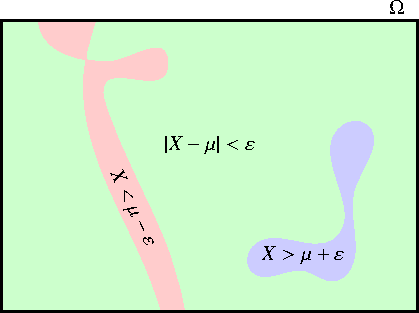
\includegraphics{images/erwartung-5.pdf}
\caption{Zur Herleitung der Tschebyscheff-Ungleichung: Ereignisse, in denen 
die Zufallsvariable um mehr als $\varepsilon$ vom Erwartungswert $\mu$
abweicht.
\label{tschebyscheff-herleitung}}
\end{figure}
\begin{figure}
\centering
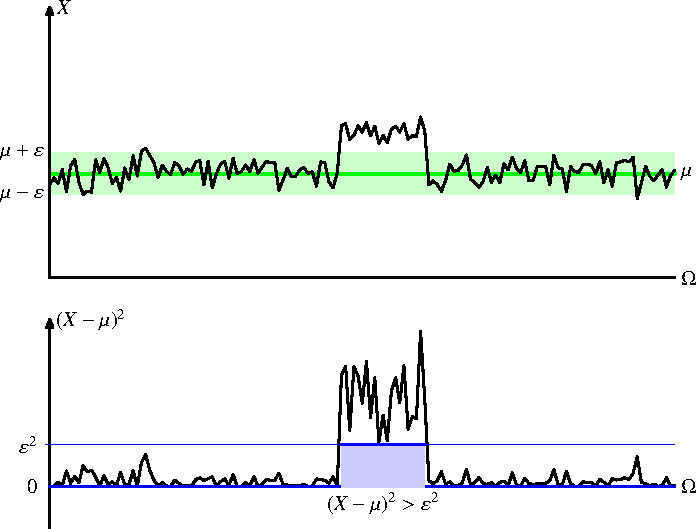
\includegraphics{images/erwartung-6.pdf}
\caption{Herleitung der Tschebyscheff-Ungleichung, charakteristische Funktion
des Ereignisses $|X-\mu|>\varepsilon$ ist blau eingezeichnet.
\label{tschebyscheff2}}
\end{figure}

\begin{satz}[Ungleichung von Tschebyscheff]
Ist eine Zufallsvariable $X$, dann lässt sich die Wahrscheinlichkeit,
dass $X$ um mehr als $\varepsilon$ vom Erwartungswert abweicht, wie
folgt abschätzen:
\[
P(|X-\mu| >\varepsilon)\le\frac{\operatorname{var}(X)}{\varepsilon^2}.
\]
\end{satz}

Lässt man $\varepsilon$ wachsen findet man, dass Abweichungen
deutlich grösser als $\sqrt{\operatorname{var}(X)}$ 
sehr unwahrscheinlich sind.

\begin{proof}[Beweis]
Sei $A =\{\omega\;|\;|X(\omega)-\mu|>\varepsilon\}$ das Ereignis, dass die
Zufallsvariable $X$ um mehr als $\varepsilon$ vom Mittelwert abgewichen
ist.
Dies ist in Abbildung~\ref{tschebyscheff-herleitung} das rote und blaue Gebiet.
Offensichtlich ist dies dasselbe, wie wenn $(X-\mu)^2$ mehr als
$\varepsilon^2$ von 0 abweicht.
Es gilt daher:
\[
\varepsilon^2 \chi_{A} \le (X-\mu)^2,
\]
wie man auch aus der Abbildung~\ref{tschebyscheff2} ablesen kann.
Wenden wir darauf den Erwartungswert an, folgt
\[
\varepsilon^2 P(A)\le E((X-\mu)^2)=\operatorname{var}(X)
\]
Die Tschebyscheffsche Ungleichung folgt jetzt nach Division durch
$\varepsilon^2$.
\end{proof}
Beispiel:
Bei der Herstellung von 1k$\Omega$ Widerständen
möchte man sicherstellen,
dass nur bei 1\% aller produzierten Widerstände der Wert um mehr als
10$\Omega$ vom Sollwert abweicht.
Um das zu überprüfen entnimmt man der
Produktion eine Stichprobe, und schätzt die Varianz ab.
Wie gross darf die
Varianz maximal werden, damit die Bedingung noch erfüllt ist?

Die Tschebyscheffsche Ungleichung liefert in diesem Fall
\[
\operatorname{var}(X)\ge\varepsilon^2P(|X-\mu| >\varepsilon)
\]
oder
\[
\operatorname{var}(X)\ge 10^2\cdot 0.01=1.
\]
Sobald die Varianz der Stichprobe grösser als 1$\Omega^2$ ist, kann die
Tschebyscheffungleichung die Einhaltung der Qualitätsvorgabe nicht
mehr garantieren.

Die Tschebyscheff-Ungleichung ist bei weitem nicht die bestmögliche.
Fragt man zum Beispiel nach der Wahrscheinlichkeit, dass $X$ um mehr
als zwei Standardabweichungen, also um mehr als $2\sqrt{\operatorname{var}(X)}$ vom
Erwartungswert abweicht, dann liefert sie
\[
P(|X-\mu|>2\sqrt{\operatorname{var}(X)})
\le\frac{\operatorname{var}(X)}{2^2\operatorname{var}(X)}=\frac14.
\]
Diese Ungleichung gilt für jede Zufallsvariable $X$.
Es gibt aber Zufallsvariablen, für die 
\[
P(|X-\mu|>2\sqrt{\operatorname{var}(X)})\le 0.05.
\]
Wir werden mit der Normalverteilung solche Zufallsvariablen kennenlernen.
Auf das Beispiel angewendet bedeutet dies, dass die Tschebyscheff-Ungleichung
möglicherweise viel zu oft behauptet, dass die Produktionsqualität ungenügend
ist, weil die Widerstandswerte vermutlich in guter Näherung normalverteilt
sein werden.

\subsection{Wie gut approximiert der Mittelwert den Erwartungswert?} \label{approximation-mittelwert}
Wir betrachten eine Folge von unabhängigen Zufallsvariablen $X_1, X_2,\dots$, die
alle den gleichen Erwartungswert $E(X_i)=\mu$ und die gleiche Varianz
$\operatorname{var}(X_i)=\sigma^2$ haben.
Dann erwartet man, dass 
der Mittelwert der ersten $n$ Zufallsvariablen, also die
Grösse
\[
M_n=\frac{X_1+X_2+\dots+X_n}{n}
\]
eine gute Näherung ist für $\mu$. Trotzdem kann es vorkommen, wegen
einzelner Ausreisser unter den $X_i$ der Mittelwert recht weit weg
vom Mittelwert liegt.
Der folgende Satz von Bernoulli sagt, wie wahrscheinlich
es ist, dass der Mittelwert weiter als $\varepsilon$ vom Erwartungswert
entfernt ist.

Zunächst halten wir fest, dass
\[
M_n=\frac{X_1+\dots+X_n}{n}
\]
eine Zufallsvariable ist mit Erwartungswert
\[
E(M_n)=E\biggl(\frac{X_1+\dots+X_n}{n}\biggr)
=\frac{E(X_1)+\dots+E(X_n)}{n}=\mu
\]
und Varianz
\[
\operatorname{var}(M_n) =\frac1{n^2}\sum_{i=1}^n\operatorname{var}(X_i)
=\frac{\sigma^2}n,
\]
wie man mit den Rechenregeln für die Varianz sofort nachrechnet.

\index{Gesetz der grossen Zahlen}
\index{Bernoulli!Gesetz der grossen Zahlen}
\begin{satz}[Bernoullis Gesetz der grossen Zahlen]
Die Wahrscheinlichkeit, dass der Mittelwert von $n$ unabhängigen Zufallsvariablen
mit Erwartungswert $\mu$ und Varianz $\sigma^2$ mehr als $\varepsilon$ von $\mu$
abweicht, ist
\[
P(|M_n-\mu|>\varepsilon)\le \frac{\sigma^2}{\varepsilon^2n}.
\]
Insbesondere gilt
\[
\lim_{n\to\infty}P(|M_n-\mu|>\varepsilon)=0.
\]
\end{satz}
\begin{proof}[Beweis]
Aus der Tschebyscheffschen Ungleichung folgt:
\[
P(|M_n-\mu|>\varepsilon)\le\frac{\operatorname{var}(M_n)}{\varepsilon^2}=
\frac{\sigma^2}{n\varepsilon^2}.
\]
Dies entspricht genau der Behauptung.
\end{proof}
Leider sind die Vorhersagen wie auch bei der Tschebyscheff-Ungleichung
nur beschränkt nützlich.
Wenn die Wahrscheinlichkeit, dass der Mittelwert
um mehr als $\sigma$ vom Erwartungswert abweicht, kleiner als 1\% sein
soll, sind dafür nach dem Gesetz der grossen Zahlen mindestens 100 Summanden
nötig.

\subsection{Wie genau ist die empirische Häufigkeit?}
Wir haben durch Wiederholung von Experimenten auch versucht, die
Wahrscheinlichkeit eines Ereignisses durch die Häufigkeit zu approximieren,
mit welcher dieses Ereignis eintritt.
Mit dem Satz von Bernoulli ist es uns jetzt auch möglich, die
Wahrscheinlichkeit dafür abzuschätzen, dass wir ein falsches
Resultat erhalten.
\begin{satz}
Wird ein Experiment $n$ mal durchgeführt, und tritt dabei das Ereignis $A$
mit der relativen Häufigkeit $h$ ein, dann ist die Wahrscheinlichkeit,
dass $h$ um mehr als $\varepsilon$ von $P(A)$ abweicht
\[
P(|h- P(A)|>\varepsilon)\le \frac{P(A)(1-P(A))}{n\varepsilon^2}
\le\frac{1}{4n\varepsilon^2}.
\]
\end{satz}
\begin{proof}[Beweis]
Wir betrachten die Zufallsvariablen $X_i$, welche den Wert $1$ hat,
wenn im $i$-ten Versuch das Ereignis $A$ eingetreten ist, und sonst $0$.
Diese Zufallsvariablen sind offensichtlich unabhängig.
Betrachtet man
nur die einzelne Durchführung $i$ des Versuches, dann ist $X_i$
die Funktion
$\chi_A$, welchen
den Erwartungswert $E(\chi_A)=P(A)$, und die Varianz ist
\begin{align*}
\operatorname{var}(\chi_A)&=E(\chi_A^2)-E(\chi_A)^2=E(\chi_A)-E(\chi_A)^2\\
&=P(A)-P(A)^2=P(A)(1-P(A))
\end{align*}
hat.
Der Mittelwert $M_n$ ist die Anzahl der Versuche, bei denen das Ereignis
$A$ eingetreten ist, geteilt durch $n$, also die Anzahl aller Versuche,
$h=M_n$.
Damit folgt aus dem Gesetz der grossen Zahlen:
\[
P(|h-P(A)|>\varepsilon)\le\frac{P(A)(1-P(A))}{n\varepsilon^2}.
\]
Die letzte Ungleichung des Satzes folgt aus der Tatsache, dass die Funktion
$p\mapsto p(1-p)=p-p^2$ bei $p=\frac12$ ein Maximum hat, also
$P(A)(1-P(A))\le\frac14$ gilt.
\end{proof}

Insbesondere verstehen wir jetzt, warum es sehr lange dauern kann, bis
wir durch Zählen der Häufigkeit eines Ereignisses dessen Wahrscheinlichkeit
auch nur auf wenige Stellen nach dem Komma bestimmen können.
Wenn wir verlangen, dass die relative Häufigkeit mit
99\% Sicherheit die Wahrscheinlichkeit auf drei Stellen annähert, also
$\varepsilon=10^{-3}$, dann müssen wir verlangen
\begin{align*}
\frac{1}{4n\varepsilon^2}&\le 0.01\\
\frac1{4\cdot 10^{-3\cdot 2}\cdot10^{-2}}=25\cdot 10^6&\le n.
\end{align*}
Der Versuch muss also mindestens 25 Millionen mal wiederholt werden,
um eine Genauigkeit von drei Stellen nach dem Komma mit 99\% Sicherheit
zu erreichen.
Dies deckt sich mit den Beobachtungen in der Würfelsimulation
in Tabelle
\ref{wuerfel-simulation}.
\begin{figure}
\centering
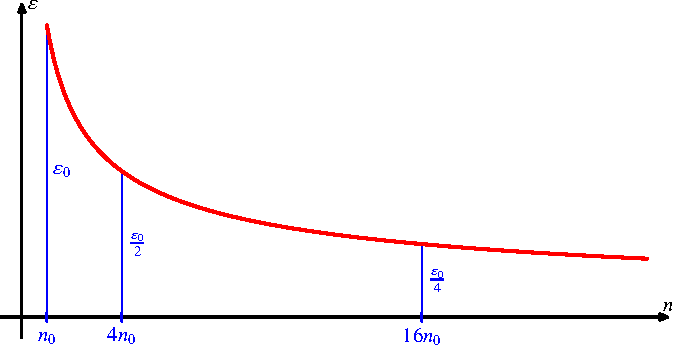
\includegraphics{images/erwartung-7.pdf}
\caption{Abnahme des Fehlers der relativen Häufigkeit mit der Anzahl
Wiederholungen.
Um den Fehler zu halbieren, muss die Anzahl der Versuche
vervierfacht werden.
\label{fehlerabnahme}}
\end{figure}
Der verbleibende Fehler der relativen Häufigkeit ist proportional zu
$\frac1{\sqrt{n}}$, wenn $n$ die Anzahl der Versuche ist.
Die Abhängigkeit des zu erwartenden Fehlers der relativen Häufigkeit mit
der Anzahl der Versuche ist in Abbildung~\ref{fehlerabnahme} dargestellt.



\section{Lineare Regression}
\index{Regression!lineare}
\index{lineare Regression}
\index{Kurvenanpassung}
\begin{figure}
\begin{center}
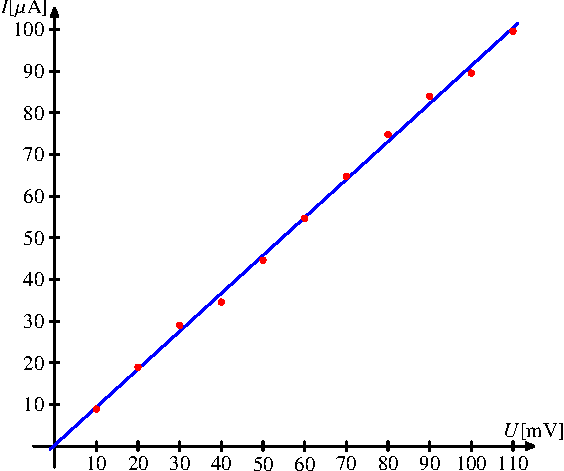
\includegraphics{images/regression-1.pdf}
\end{center}
\caption{Anpassung einer Geraden an gemessene
Strom-/Spannungswerte\label{ohm-regression}}
\end{figure}
Der Satz \ref{erwartungswert-charakterisierung} hat gezeigt, dass der
Erwartungswert jener Wert ist, der die Varianz minimiert.
Diese Idee
lässt sich auch auf kompliziertere Zusammenhänge anwenden.
In einem
Stromkreis erwartet man auf Grund des Ohmschen Gesetzes, dass Spannung $U$
und Strom $I$ proportional sind: $U=RI$.
Führt man eine Messung von beiden
Grössen durch, erhält man zwei Zufallsvariablen $U(\omega)$ und $I(\omega)$,
und die Proportionalität wird wegen der Messfehler meistens nicht mehr
erfüllt sein.
Wie gross ist der Widerstandswert $R$? Es wäre zwar denkbar,
für jede Messung den Widerstandswert zu errechnen, und dann das Mittel
zu bilden.
Noch besser ist aber, den Widerstandswert $R$ so zu bestimmen,
dass der erwartete quadratische Fehler
$E( (U-RI)^2)$
möglichst klein ist.
Abbildung \ref{ohm-regression} zeigt eine solche Gerade.


\subsection{Regressionsgerade}
Etwas allgemeiner finden wir folgenden Satz über die sogenannte
Regressionsgerade:
\begin{satz}
\label{rekursion}
Seien $X$ und $Y$ zwei reelle Zufallsvariablen.
Die Gerade mit der
Gleichung $y=ax+b$ minimiert die Varianz
$\operatorname{var}(aX+b-Y)$ genau dann, wenn 
\begin{align*}
a
&=
\frac{E(XY)-E(X)E(Y)}{(E(X^2)-E(X)^2)}=\frac{\operatorname{cov}(X,Y)}{\operatorname{var}(X)},
\\
b
&=
E(Y)-E(X)a.
\end{align*}
\end{satz}
\begin{proof}[Beweis]
Der mittlere quadratische Fehler ist
\begin{align*}
Q(a,b)&=E((aX+b-Y)^2)\\
&=E(a^2X^2+b^2+Y^2+2abX-2aXY -2bY)\\
&=a^2E(X^2)+b^2+E(Y^2)+2abE(X)-2aE(XY)-2bE(Y).
\end{align*}
Um das Minimum zu finden, setzen wir die partiellen Ableitungen nach $a$
und $b$ gleich Null, und finden:
\begin{align*}
0=\frac{\partial Q}{\partial a}&=2aE(X^2)+2bE(X)-2E(XY)\\
0=\frac{\partial Q}{\partial b}&=2b+2aE(X)-2E(Y).
\end{align*}
Dies ist gleichbedeutend mit dem folgenden linearen Gleichungssystem für
die Koeffizienten
$a$ und $b$
\begin{alignat*}{4}
E(X^2)a\,&+\,&E(X)b\,&=\,&E(XY)\\
E(X)a\,&+&b\,&=&E(Y).
\end{alignat*}
Multipliziert man die zweite Gleichung mit $E(X)$ und subtrahiert sie von der
ersten, erhält man eine Gleichung für $a$:
\begin{align*}
(E(X^2)-E(X)^2)a&=E(XY)-E(X)E(Y)\\
a&=\frac{E(XY)-E(X)E(Y)}{(E(X^2)-E(X)^2)}.
\end{align*}
Aus der zweiten Gleichung kann man nun auch $b$ finden:
\[
b=E(Y)-E(X)a,
\]
womit alles bewiesen ist.
\end{proof}
Die Gleichung für $b$ hat eine unmittelbare Konsequenz: die Regressionsgerade
geht immer durch den Punkt $(E(X), E(Y))$.
In der Tat, damit der Punkt
$(E(X), E(Y))$ auf der Geraden liegt, muss die Bedingung $E(Y)=aE(X)+b$
erfüllt sein.
Schafft man $aE(X)$ auf die linke Seite, wird daraus

$E(Y)-aE(X)=b$, also genau die Gleichung für $b$.

\subsubsection{Der mittlere quadratische Fehler}
Der mittlere quadratische Fehler lässt sich natürlich auch berechnen.
Wir sind von $\operatorname{var}(Y-aX-b)$ als zu optimierender
Grösse ausgegangen.
Inzwischen haben wir $a$ und $b$ bestimmt,
also können wir auch den Fehler berechnen.
Dazu sind die Rechenregeln
hilfreich:
\begin{align*}
\operatorname{var}(Y-aX-b)
&=
\operatorname{var}(Y) + 
\operatorname{var}(-aX) + 
\operatorname{var}(-b)
+2\operatorname{cov}(-aX,Y)
\\
&=
\operatorname{var}(Y)+a^2\operatorname{var}(X)-2a\operatorname{cov}(X,Y)
\\
&=
\operatorname{var}(Y)
+ \frac{\operatorname{cov}(X,Y)^2}{\operatorname{var}(X)^2}\operatorname{var}(X)
-2 \frac{\operatorname{cov}(X,Y)}{\operatorname{var}(X)}\operatorname{cov}(X,Y)
\\
&=
\operatorname{var}(Y)-\frac{\operatorname{cov}(X,Y)^2}{\operatorname{var}(X)}.
\end{align*}
Im zweiten Schritt mussten wir die Formel (\ref{var-summe-abhaengig})
verwenden, da die Zufallsvariablen $X$ und $Y$ nicht unabhängig sind.

Natürlich
ist der Fehler 
wahrscheinlich ungefähr proportional zur Varianz der $Y$-Werte,
ohne Varianz gibt's auch keinen Fehler.
Wir versuchen daher den Term
$\operatorname{var}(Y)$ auszuklammern:
\begin{align*}
\operatorname{var}(Y-aX-b)
&=
\operatorname{var}(Y)\left(1-\frac{\operatorname{cov}(X,Y)^2}{\operatorname{var}(X)\operatorname{var}(Y)}\right).
\end{align*}
Der Bruch wird damit ein natürliches Qualitätsmass für die Regressionsgerade:
\begin{definition}
Der Quotient
\[
r=\frac{\operatorname{cov}(X,Y)}{\sqrt{\operatorname{var}(X)\operatorname{var}(Y)}}
\]
heisst Regressionskoeffizient.
\end{definition}

\begin{figure}
\centering
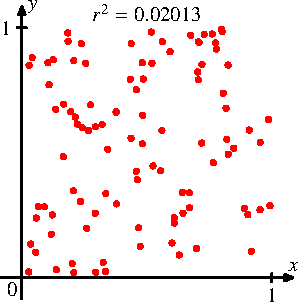
\includegraphics{images/regression-2.pdf}\;
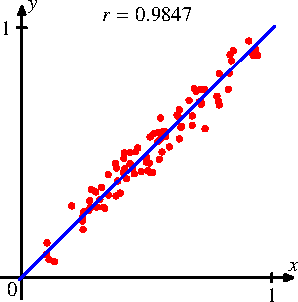
\includegraphics{images/regression-3.pdf}\;
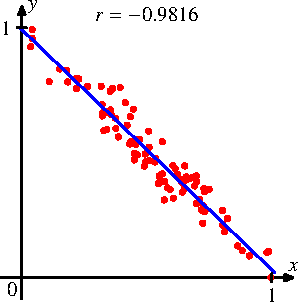
\includegraphics{images/regression-4.pdf}
\caption{Aussehen der Punktwolke für verschiedene Werte des Regressionskoeffizienten.
Für $r\simeq 0$ besteht keine Abhängigkeit zwischen den Variablen, $r\simeq 1$
zeigt eine gute, positive Abhängigkeit an, $r\simeq -1$ eine starke
negative Abhängigkeit.
\label{regressionskoeffizient-graphik}}
\end{figure}

Die Regression ist also umso genauer, je näher $r$ bei $\pm 1$ liegt.
Ausserdem hat $r$ immer das gleiche Vorzeichen wie die
Steigung der Regressionsgeraden.
Dies ist in Abbildung~\ref{regressionskoeffizient-graphik} dargestellt.

\subsubsection{Berechnung aus empirischen Daten}
Auch die Koeffizienten der Regressionsgeraden sind mit einfachen Formeln
zu bestimmen, wenn man nur Messwerte, deren Quadrate und das Produkt summiert:
\begin{align*}
a
&=
\frac{\displaystyle n\sum_{i=1}^nx_iy_i-\sum_{i=1}^nx_i\sum_{i=1}^ny_i}{\displaystyle n\sum_{i=1}^nx_i^2-\biggl(\sum_{i=1}^nx_i\biggr)^2},\\
b
&=
\frac1n\sum_{i=1}^ny_i-a\frac1n\sum_{i=1}^nx_i,\\
r^2
&=
\frac{
\displaystyle
\biggl(n\sum_{i=1}^n x_iy_i-\sum_{i=1}^n x_i\sum_{i=1}^ny_i\biggr)^2
}{
\displaystyle
\biggl(n\sum_{i=1}^nx_i^2-\biggl(\sum_{i=1}^nx_i\biggr)^2\biggr)
\biggl(n\sum_{i=1}^ny_i^2-\biggl(\sum_{i=1}^ny_i\biggr)^2\biggr)
}.
\end{align*}

\subsection{Anwendungsbeispiel}
\begin{table}
\begin{center}
\begin{tabular}{|c|c|}
\hline
Zeit [s]&Länge [mm]\\
\hline
6&10.98\\
10&13.89\\
14&16.23\\
18&18.57\\
\hline
\end{tabular}
\end{center}
\caption{Länge der Verzögerungselemente für K1100T in Abhängigkeit von der
Verzögerungszeit\label{delaylengths}}
\end{table}
Modellraketenmotoren auf Feststoffbasis verwenden ein Verzögerungselement,
welches nach Abbrand des eigentlichen Treibsstoffs noch einige Sekunden
weiter brennt, um dann eine Schwarzpulverladung zu zünden, die einen Fallschirm
auswerfen kann.
Die Verzögerungselemente werden nur für wenige, diskrete
Verzögerungszeiten hergestellt.
Ist kein passendes Verzögerungselement
verfügbar, muss
ein längeres Verzögerungselement durch Verkürzung auf die passende
Verzögerungszeit eingestellt werden.
Dazu muss jedoch der Zusammenhang
zwischen Verzögerungszeit und Länge des Elementes bekannt sein.
Der Hersteller macht die Angaben in Tabelle \ref{delaylengths}.

\subsubsection{Berechnung von Hand}
Die Berechnung auf dem Papier kann man zum Beispiel mit Hilfe
des Berechnungsschemas gemäss folgender Tabelle
organisieren, welche auch alle relevanten Formeln zeigt:
\begin{center}
\begin{tabular}{|l|l|l|l|}
\hline
$E(T)$&&&\\
$E(T^2)$&\footnotesize$\operatorname{var}(T)=E(T^2)-E(T)^2$&&\\
\hline
$E(L)$&&&\\
$E(L^2)$&\footnotesize$\operatorname{var}(L)=E(L^2)-E(L)^2$&&\\
\hline
$E(TL)$&\footnotesize$\operatorname{cov}(T,L)=E(TL)-E(T)E(L)$&$a=\frac{\operatorname{cov}(T,L)}{\operatorname{var}(T)}$&\footnotesize$b=E(L)-aE(T)$\\
&&$r=\frac{\operatorname{cov}(T,L)}{\sqrt{\operatorname{var}(T)\operatorname{var}(L)}}$&\\
\hline
\end{tabular}
\end{center}
Die Durchführung der Rechnung führt zu folgendem Resultat:
\begin{center}
\begin{tabular}{|r|r|r|r|}
\hline
12.0000&&&\\
164.0000&20.0000&&\\
\hline
14.9175&&&\\
230.4376&7.9058&&\\
\hline
191.5650&12.5550&0.627750&7.38450\\
&&0.998456&\\
\hline
\end{tabular}
\end{center}
Somit kann man als Näherungsformel für die Länge des Verzögerungselements
die lineare Funktion
\[
l=0.62775 \cdot t+7.3845
\]
verwenden.
Der mittlere quadratische Fehler dieser Näherung ist
\[
\Delta = \operatorname{var}(L)(1-r^2)=0.024.
\]
Der Längenfehler ist also etwa $\sigma_L=\sqrt{0.024}=0.15$mm, was einer
Ungenauigkeit der Verzögerungsdauer von 0.25s entspricht.
Angesichts
der Fertigungs- und Betriebs\-toleranzen von bis zu 20\%, verursacht durch
Schwankungen in Abmessungen, physikalischen Eigenschaften des Treibstoffs
und Temperatur beim Abbrand ist dies bei weitem genau genug.
\subsubsection{Berechnung mit R}
\begin{figure}
\begin{center}
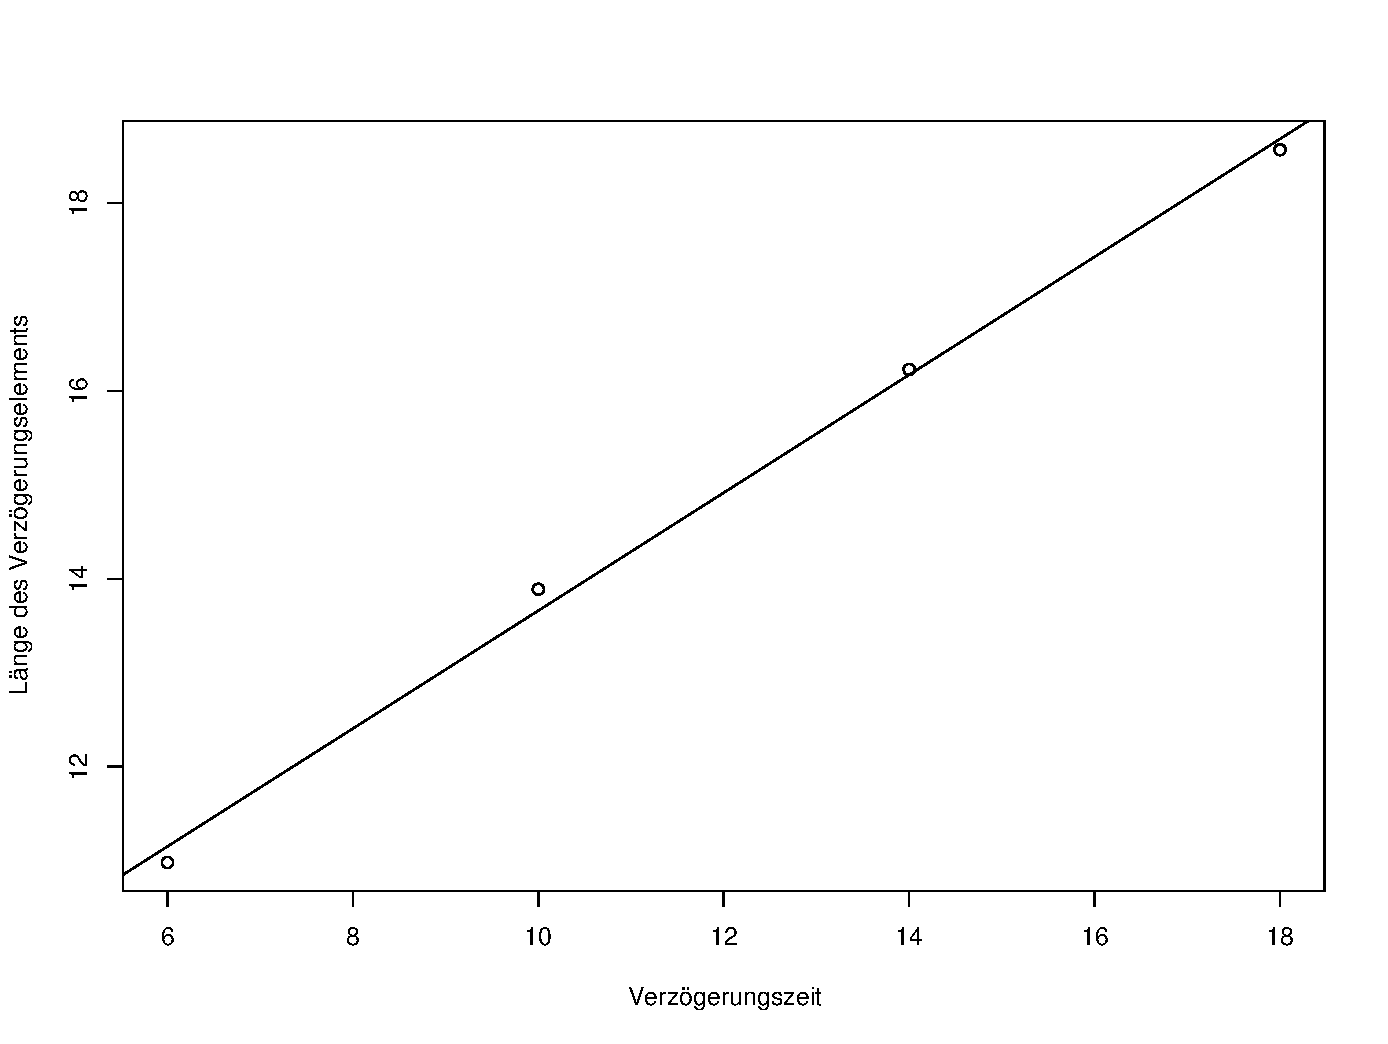
\includegraphics[width=0.7\hsize]{graphics/verzoegerungszeit}
\end{center}
\caption{Von R erzeugte graphische Darstellung der Regressionsgerade
für die Verzögerungszeit\label{verzoegerungszeit}}
\end{figure}
Die Software R
ist ein leistungsfähiges freies Softwarepaket für statistische
Berechnungen.
Mit folgenden Befehlen kann das obige Regressionsproblem
mit R gelöst, und die Graphik \ref{verzoegerungszeit} dargestellt
werden:

{\footnotesize
\begin{verbatim}
> zeit = c(6,10,14,18)
> laenge = c(10.98, 13.89, 16.23, 18.57)
> laenge.lm = lm(laenge ~ zeit)
> summary(laenge.lm)

Call:
lm(formula = laenge ~ zeit)

Residuals:
     1      2      3      4 
-0.171  0.228  0.057 -0.114 

Coefficients:
            Estimate Std. Error t value Pr(>|t|)   
(Intercept)  7.38450    0.31608   23.36  0.00183 **
zeit         0.62775    0.02468   25.43  0.00154 **
---
Signif. codes:  0 `***' 0.001 `**' 0.01 `*' 0.05 `â'0.1 ` ' 1 

Residual standard error: 0.2208 on 2 degrees of freedom
Multiple R-Squared: 0.9969,	Adjusted R-squared: 0.9954 
F-statistic: 646.9 on 1 and 2 DF,  p-value: 0.001542 

> plot(laenge ~ zeit, xlab="Verzoegerungszeit",
  ylab="Laenge des Verzoegerungselements")
> abline(laenge.lm)
\end{verbatim}
}
R kann von \url{https://www.r-project.org} heruntergeladen werden.
